% Grobe  Architekturbeschreibung  durch  Bausteine/Komponenten  (Kein  detailliertes Klassendiagramm).
\section{Systemübersicht}
Die Systemarchitektur wird durch einen Modularen Ansatz umgesetzt.
Die einzelnen Module sind durch ihre Aufgabenbereiche getrennt.
Bei den einzelnen Modulen wird intern zwischen Steuerung, Anzeige und Daten aufgeteilt.
Es wird in folgende 6 Module aufgeteilt:

\begin{itemize}
\item Workflow
\item I/O
\item Visualisierung
\item Logger
\item Einstellungen
\item Interaktion
\end{itemize}
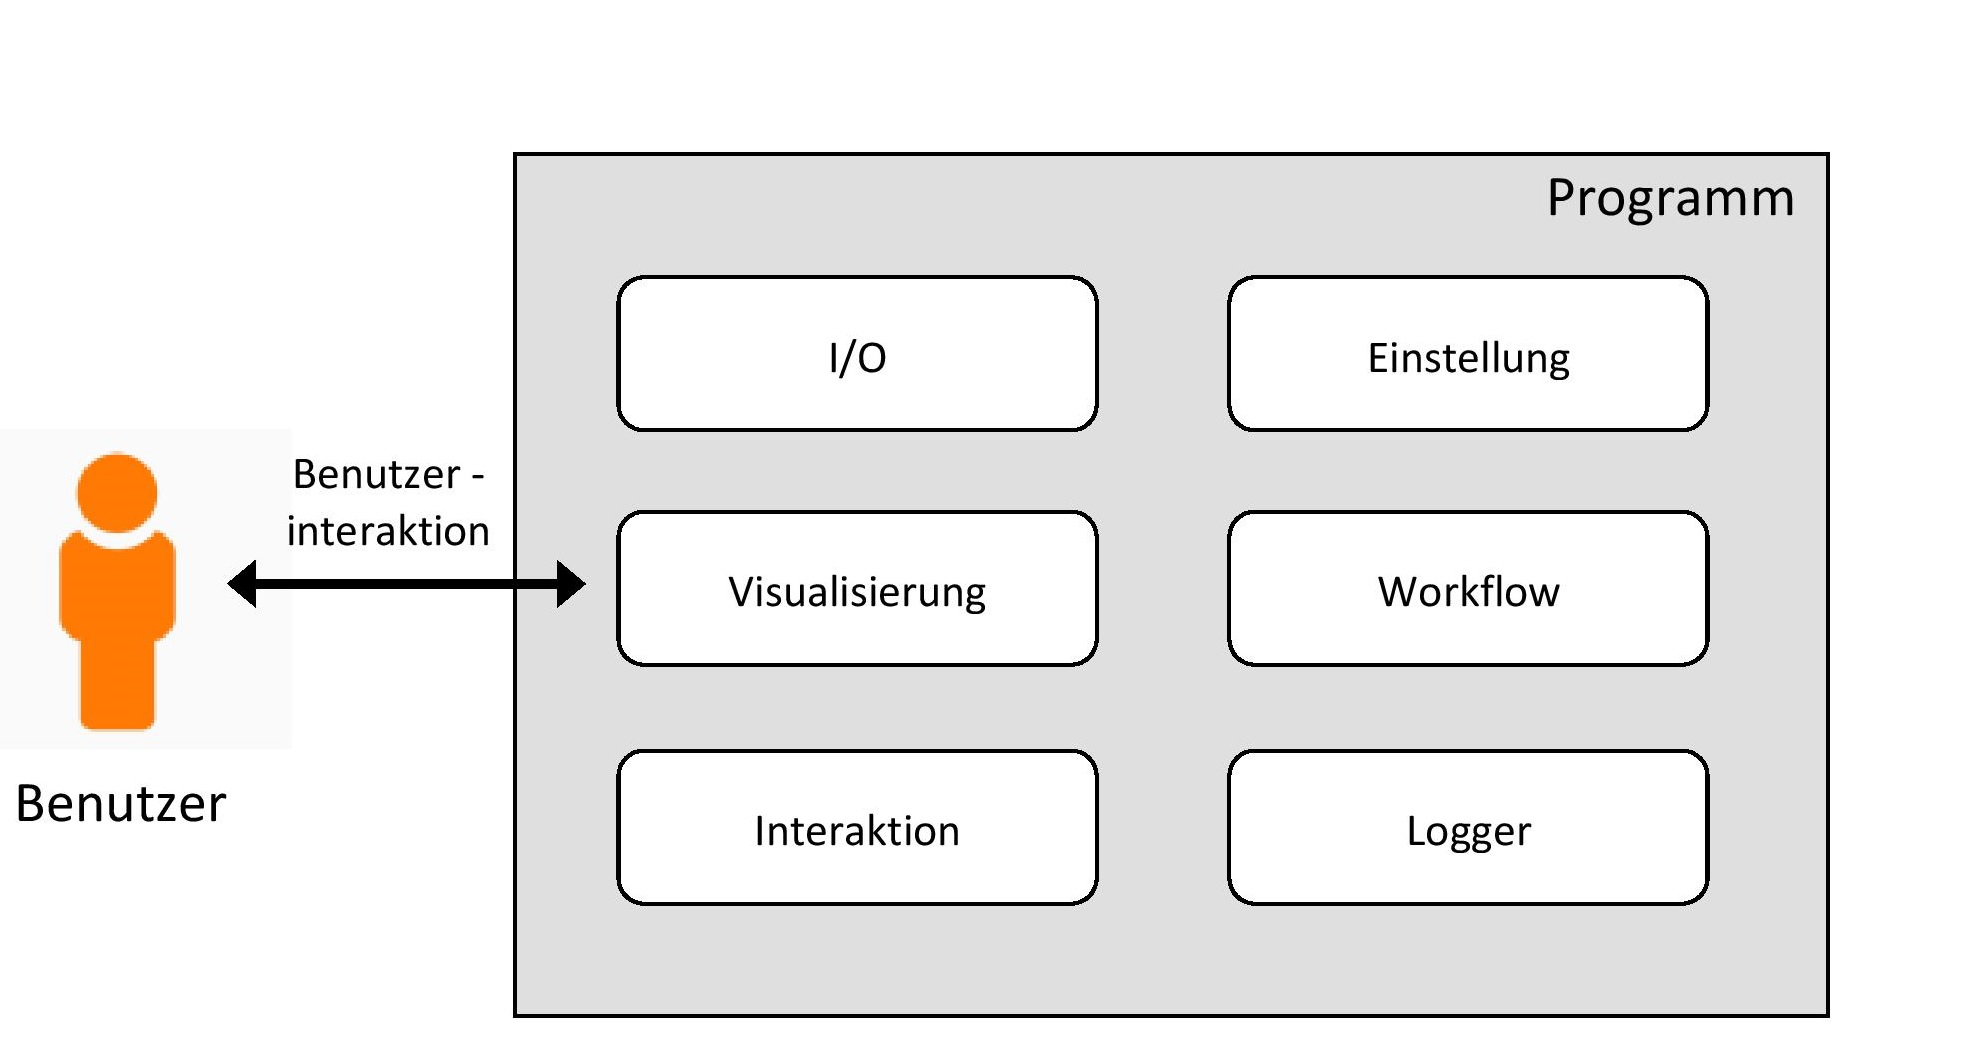
\includegraphics[scale=0.35]{img/Uebersicht.jpg} 

\newpage 
\section{Module}
Im weiteren folgt eine kurze Definition der Module.

\subsection{Workflow}
Das Modul Workflow bietet mindestens einen Workflow an und bündelt alle Workflowspezifischen
Einstellungen und Auswahlmöglichkeiten, inklusive:

\begin{itemize}
\item Workflows wie den 4-Phasen-Workflow
\item Speichern und laden von Wokflowkonfigurationen
\item Algorithmenauswahl für jede Phase 
\end{itemize}

\subsection{I/O}

Das Modul I/O bietet Funktionen für die Ein- und Ausgabedaten an, inklusive:

\begin{itemize}
\item Einlesen und übergeben von Einzelbilder
\item Speichern von (Zwischen-) Ergebnissen
\end{itemize}

\subsection{Visualisierung}
Das Modul Visualisierung bietet Anzeigen der (Zwischen-) Endergebnissen  an, inklusive:

\begin{itemize}
\item Anzeigen der Ausgabedaten der (Zwischen-) Ergebnisse
\item optional, Manipulation der Ausgangsdaten der (Zwischen-) Ergebnisse
\end{itemize}

\subsection{Logger}
Das Modul Logger stellt Logs bereit, inklusive:

\begin{itemize}
\item Info, Warning, Error, Debug
\item Anzeige und Abspeichern dieser Logs
\end{itemize}

\subsection{Einstellung}
Das Modul Einstellungen behandelt (globale) lokale Einstellungen, inklusive:

\begin{itemize}
\item Speichern und Laden von Einstellungen einzelner Verfahren
\end{itemize}

\subsection{Interaktion}
Das Modul Interaktion behandelt Benutzereingaben innerhalb des Programms, inklusive:

\begin{itemize}
\item Starten und Stoppen, Arbeitsindikator 
\end{itemize}

\newpage 
\section{Datenflussübersicht}

Dieses Diagramm stellt eine Grobübersicht über den Datenfluss zwischen den Einzelnen Modulen dar.
Diese sind nur als grobe Orientierung anzusehen und werden im Entwurf und in der Implementierung möglicherweise auf andere Weise umgesetzt.
\begin{normalsize}

\end{normalsize}
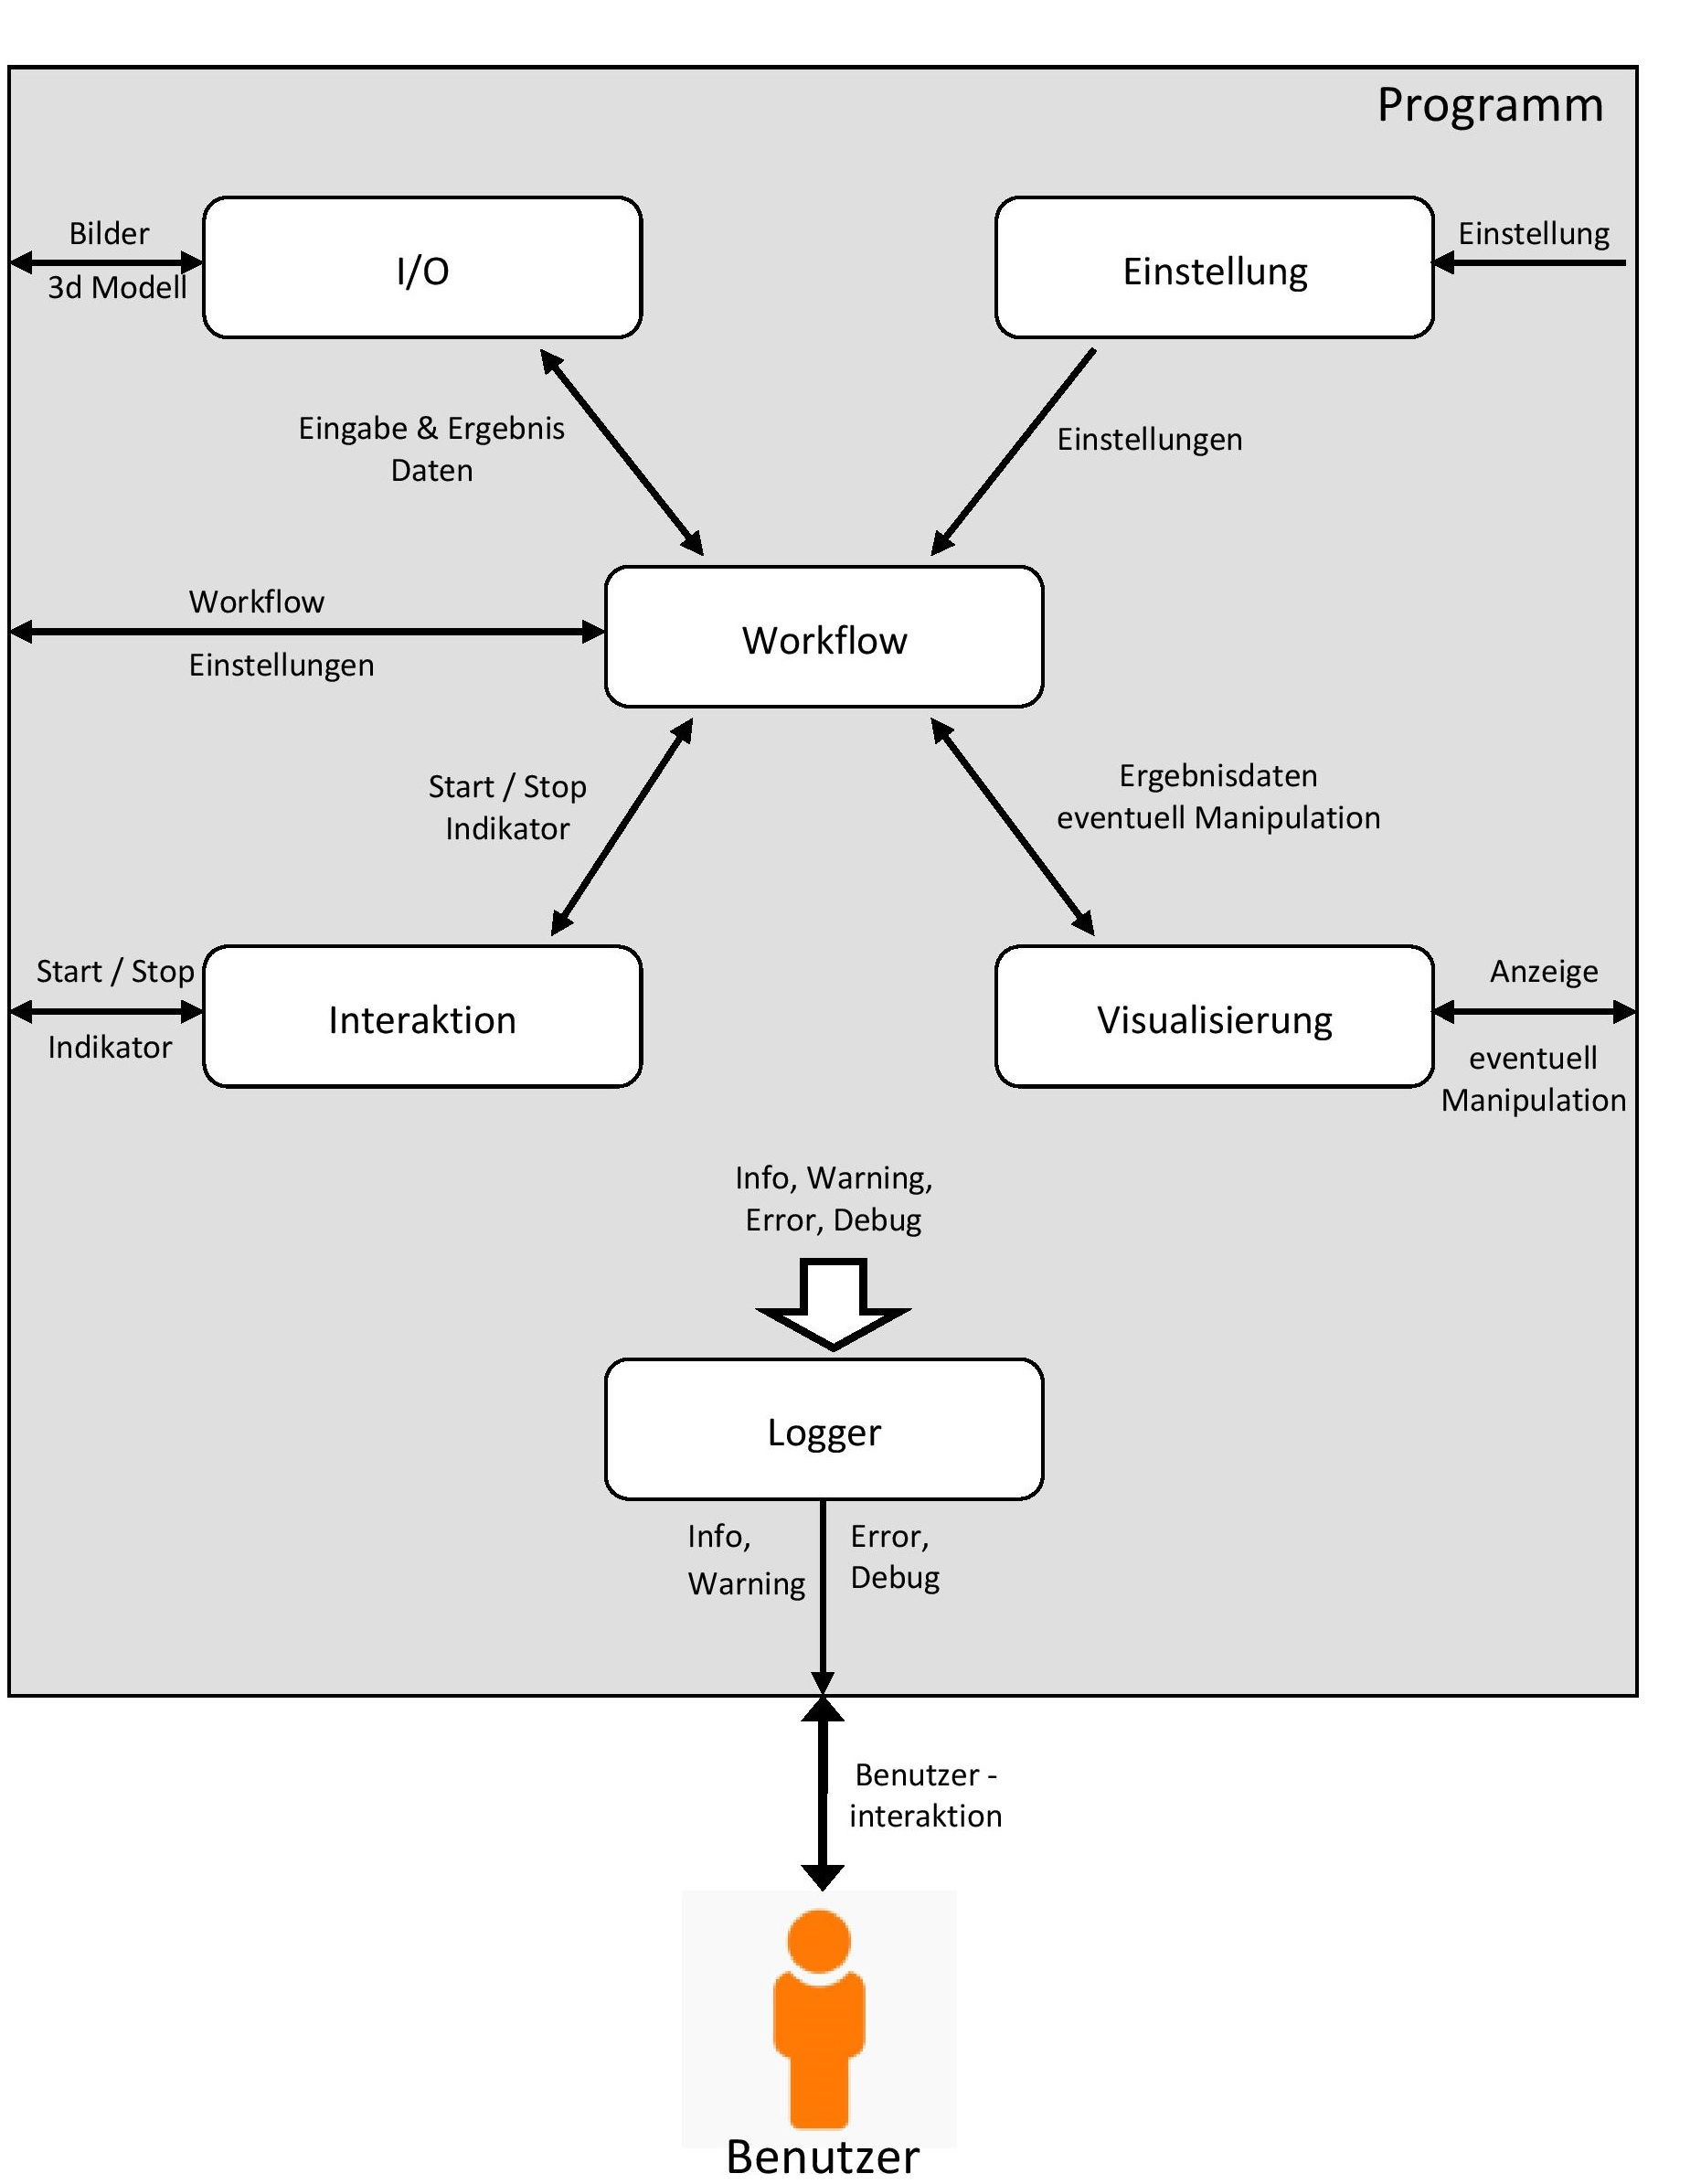
\includegraphics[scale=0.5]{img/Datenflussuebersicht.jpg} 
\newpage 
\section{Anwendugsfälle mit Sequenzdiagramm}
\subsection{Anwendugsfall: Rekonstruktion aus unzusammenhängenden Einzelbilder}
Gegeben: Vielzahl an Einzelbilder einer Szene die nicht von der selben Kamera oder Position aufgenommen wurden.
Ziel: Rekonstruktion der Szene oder eines einzelnen Objektes.
Vorgehen:
\begin{itemize}
\item 1. Feature Detektor: In den Bildern wird automatisch nach „markanten“ Punkten gesucht, die hohen Wiedererkennungswert haben.\item 2. Feature Matching: Die gefundenen „markanten Punkte“ in zwei Bildern werden verglichen und einander zugeordnet.\item 3. Posenschätzung: Aus den Punktzuordnungen von zwei oder mehr Bildern werden die Positionen der Kameras ermittelt, von denen aus die Bilder aufgenommen wurden.\item 4. Tiefenschätzung: Mit Hilfe der Kamerapositionen werden die Tiefen in den Bildern trianguliert. Dadurch werden die Entfernungen der Objekte auf den Bildern bestimmt.\item 5. Modellerzeugung: Die Einzelansichten werden zu einem kompletten 3D Modell zusammengesetzt.
\end{itemize}
Stellschrauben:
\begin{itemize}
\item 1. Der Feature Detektor kann ausgewechselt werden (z. B. SIFT oder SURF)\item 2. Das Feature Matching kann auf verschiedene Arten durchgeführt werden (z. B. RANSAC oder MLESAC, jeweils mit verschiedener Initialisierungen)
\end{itemize}
\includegraphics[scale=0.5]{img/Sequez_RauE.jpg} 
\subsection{Anwendugsfall: Structure-from-Motion (SfM)}

Gegeben: Videosequenz einer Szene, mit eigenbewegung der Kamera.
Ziel: Rekonstruktion der Szene oder eines einzelnen Objektes.

Structure-from-Motion (SfM) ist ein Verfahren zur 3D-Rekonstruktion mit nur einer Kamera. Dabei wird bei SfM das 3D-Modell aus einem Video, also einer Reihe von Einzelbildern rekonstruiert. Dabei ist es wichtig, dass das Video nicht von einer statischen Position aus aufgenommen wird, vielmehr sollte die Kamera sich dabei mit Blick auf die zu rekonstruierende Szene bewegen. Bei der Rekonstruktion mittels SfM werden zwei oder mehr Einzelbilder der Eingangssequenz herangezogen, für die angenommen wird, dass sie dieselbe Szene aus verschiedenen Blickrichtungen betrachten und die Szene zwischen den Einzelbildern statisch (unverändert) geblieben ist.
Vorgehen:
\begin{itemize}
\item 1. Feature Detection: Ermitteln leicht verfolgbarer markanter Bildpunkte\item 2. Feature Tracking: Verfolgen der markanten Bildpunkte\item 3. Posenschätzung: Bestimmen der Aufnahmepunkte, Verfolgen der Kamerafahrt\item 4. Tiefenschätzung: Bestimmen der Tiefe mit lokalen Optimierungsverfahren\item 5. Modellerzeugung: Die Einzelansichten werden zu einem kompletten 3D Modell zusammengesetzt
\end{itemize}
\includegraphics[scale=0.5]{img/Sequez_SfM.jpg} 